\section{Implementation} \label{sec:impl}
In this section, we present the implementation details of the \module and the \cache based on Xen (the hypervisor) and Linux (the guest kernel).

\subsection{\name Module}
\begin{figure}[ht]
\centering
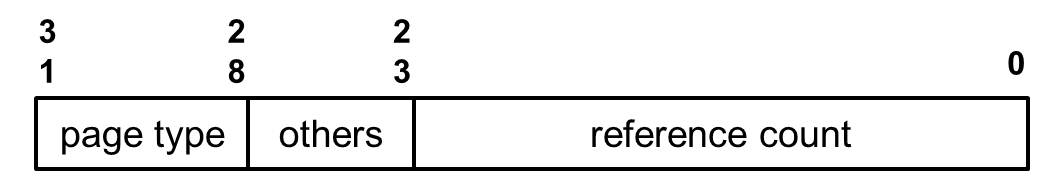
\includegraphics[width=0.45\textwidth]{image/implementation/field-of-page-type-info.jpg} \\
\caption{The layout of the traditional data structure for page type.}
\label{fig:field-of-page-type-info}
\end{figure}
The first main task of the \module is to extend the existing data structure to support semi-writable page.
As illustrated in Figure~\ref{fig:field-of-page-type-info}, the data structure for labelling page types occupies 32bits, i.e., bits 28 - 31 are allocated for page type, bits 23 - 27 is for others (e.g., bit 26 indicate if this page has been validated), and bits 0 - 22 are for reference count of one page type.
The existing page types have occupied all page type bits, and there is no extra bit available for semi-writable page.
Facing this problem, we do not choose to introduce new data structures, as it would increase the management complexity and result in many modifications of all related management functions.
Instead, we choose to borrow a bit from \emph{reference count}.
In particular, the \emph{reference count} field has 23 bits, recording the number of type references for a page as its current type.
%presenting how many references on a page.
In fact, the system usually does not build so many references (i.e., $2^{23}-1$) to one page. Thus, we borrow the highest bit (bit 22) as the semi-page table bit (as illustrated in Figure~\ref{fig:field-of-semi-type}).
As a consequence, it still supports more than 4 million reference counts, enough for almost all cases.
Actually, the hypervisor with \name is functioning well in our experiments.

The \module also needs to patch the page type checking functions, e.g., \_\_get\_page\_type, to adjust the checking logic.
The added checking logic is straightforward, such that we only add or change 166 SloC to achieve the whole patch.
In addition, some validation steps (e.g., DMA validations) necessary in the traditional design could be skipped when the newly introduced semi-writable page is involved in the page type update, simplifying the whole validation logic in a certain level.

\begin{figure}[ht]
\centering
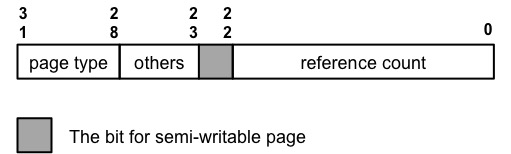
\includegraphics[width=0.45\textwidth]{image/implementation/field-of-semi-type.jpg} \\
\caption{The semi-writable page type support.}
\label{fig:field-of-semi-type}
\end{figure}

\subsection{\name Cache}
%data structures
There are three-level of the guest page table, and the \cache maintains a single-linked list for each of them.
Each node of the list has a pointer pointing to the next node and a page ID that is the base address of a cached page.
Note that this address should be a physical address, rather than a virtual address, because physical address of a page is unique in the whole system but its virtual addresses could be multiple.
Thus, using virtual address would lead to the confusion of the page type tracing and the semi-writable page management.
As the page table allocations and deallocations could happen at any time on any core, each list has its own lock to support concurrent updates.

%interfaces
The \cache has two interfaces for the runtime page table allocations and deallocations.
The \emph{pop} interface is for the page table allocations.
When this interface is invoked, the \cache fetches the top node of the corresponding list, extracts the base address of the cached page, and then returns it to the caller.
Correspondingly, the \emph{push} interface is serving the page table deallocations.
In the \emph{push} interface, the \cache saves the base address of the deallocated page into a node, and inserts it onto the top of the list.
Obviously, the \emph{pop} and \emph{push} interfaces are extremely fast as they could response the requests in a constant time.
In addition, the \cache also exports an interface for the memory management daemon for explicitly shrinking the cached pages.

%provide interfaces for end user
The \cache also adds several virtual files in \emph{sysfs}~\cite{love2004linux,mochel2005sysfs} that is a virtual file system provided by the Linux kernel.
By using the virtual files, the end user could send commands to the \cache,  as well as query and configure the internal status.
In the current implementation, we only support one command, which is able to activate and deactivate the cache service in an on-demand way.
In addition, the end user could read and write the virtual files to query the number of the cached pages, and dynamically shrink the cache size.
For instance, the end user could explicitly ask the \cache to release all the cached pages by setting the number of the cached pages to be zero.

% handle cache shrinking and page type update
The \cache mediates all page type updates related to the semi-writable pages.
For each page type update, the \cache would issue the hypercall exported by the \module to explicitly inform the hypervisor to perform security validations.
In certain cases, such as shrinking the cached semi-writable pages to writable pages, the \cache could submit a batch of requests in one hypercall.
In such case, the hypervisor would update the I/O page tables as well as flush IOTLBs at one time, saving time of the cache shrinking.

% shrinking parameters






